\section{Feature Extraction} \label{sec:featureextract}
The binary blob mask of an object contains too much redundant information for the tracking algorithm. As reviewed in \autoref{ch:review}, a binary blob could be represented as a feature vector of the centroid and the size, denoted as \autoref{eq:blobdenote1}, where $C$ is the 2D coordinate of the geometry center and $S$ is the total pixel number of the blob.
\begin{equation}\label{eq:blobdenote1}
  B = \{C,S\}
\end{equation}

This basic representation is sufficient for a single object tracking because the centroid is a unique feature for a blob. However, when two objects overlap and their blob masks merge together, they will be regarded as one single blob and therefore have only one shared centroid. The uniqueness of the centroid no longer holds, and the one-to-one matching relation between an object and its corresponding blob mask is broken.
\autoref{fig:blobmerge} shows an example demonstrating how the merged blobs impede the feature extraction. In the first two frames where two blobs are not merged, their centroids remain unique and transit a small distance from the last frame. The size of the blobs remain similar as in the last frame. In the third frame, the blobs are merged, their centroids disappear and are replaced with a single centroid at the center of two blobs. Viewing the extracted feature only, we may only conclude that there is one blob with twice the size as before. Furthermore, the location of the centroid jumps abruptly, not close to either centroids in the last frame. In the fifth frame, the blobs are again separated. An abrupt change in centroid position takes place again.

Since the tracker match objects with its nearest neighbour in the last frame, a distance that is too long will break the matching. Even if the blobs are successfully matched, a shared centroid will bring ambiguity to the label assignment. Labels may be exchanged between two objects after splitting.
\begin{figure}
  \centering
  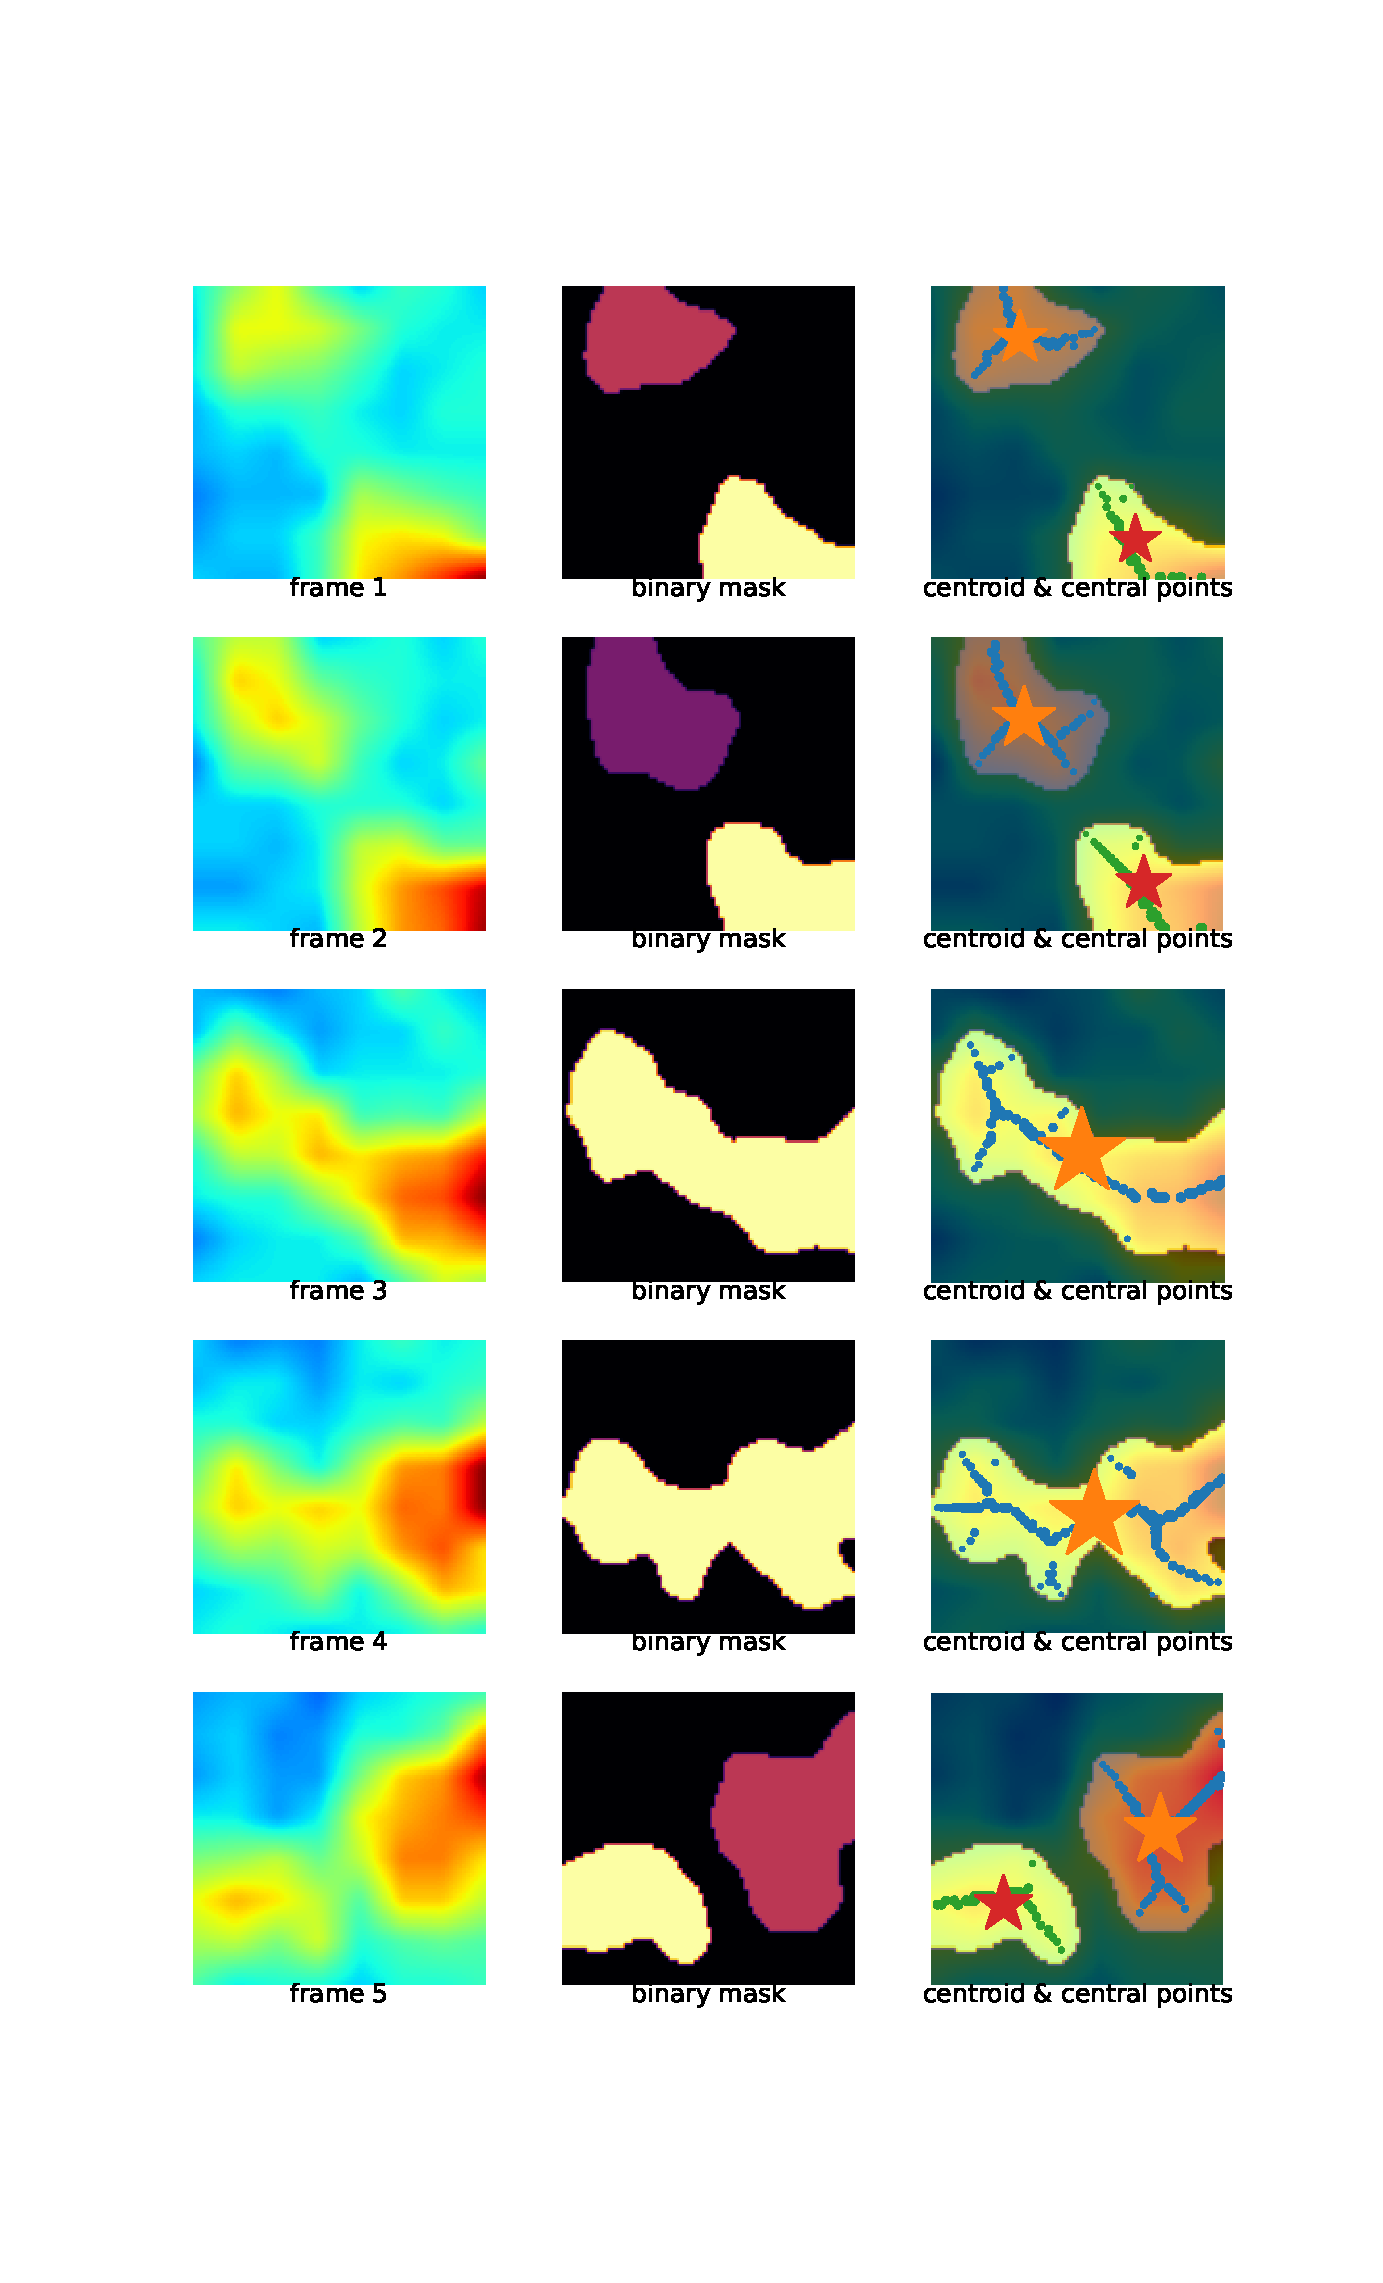
\includegraphics[width=0.6\textwidth]{figures/blobmerge.eps}
  \caption{An example frame sequence showing the blob merging issue. Left column is the interpolated image, middle column is the blob mask and right column shows the extracted feature. The star symbol represents the centroid location and the size of the star represents the size of the blob. Other round dots scattered inside the blob represent central points.}\label{fig:blobmerge}
\end{figure}

We follow the research of \cite{sharma2012blob}, adding ``central points'' as additional feature for blob representation. Central points of a blob are those points that are far away from the background, they can be found out by picking local maxima in a distance transform of the blob mask.
\subsection{Distance Transformation}
A distance transform of a binary image labels every pixel of the image by the distance between that pixel and the nearest background pixel \cite{bailey2004efficient}, which could be denoted as \autoref{eq:distancetransform}.
\begin{equation}\label{eq:distancetransform}
  I_d(x,y) = \left\{\begin{array}{cc}
               0 & I(x,y)\in\{Bg\} \\
               \min\left(\Vert x-x_0,y-y_0\Vert\right),\forall I(x_0,y_0)\in Bg & I(x,y)\in\{Ob\}
             \end{array}\right.
\end{equation}
The $\Vert\cdot\Vert$ symbol is a distance definition, could be $L_1$, $L_2$, $L_{max}$ or any other distance metric. To our concern, the distance is measured in Euclidean metric, namely $\Vert x,y\Vert=\sqrt{x^2+y^2}$.

A precise computation of the Euclidean distance transform is complex. A commonly used approximation is the chamfer distance transform \cite{butt1998optimum}. The chamfer distance transform exploits the fact that the distance between of each pixel to its nearest background pixel depends on the previously computed neighbour. The whole distance transform image could be obtained in two passes, one propagating from the upper-left corner to the lower-right corner and the other reversely. Mathematically, the two-pass algorithm with a $3\times3$ window could be written as \autoref{eq:chamferDT}, where $r,c$ denote the row and column coordinate of a pixel respectively, $x_-$ is the distance transform value after the first pass and $x_+$ is the final value after the second pass.

At the first pass, a pixel's distance to the background is propagated from three pixels above it and the one on the left of it. Two vertical and horizontal connected pixel contribute to the transform value by an distance increment of $a$, while two diagonal connected pixel contribute and increment by $b$. The value $a$ and $b$ depend on the desired approximation and usually $a\le b$. The transform result of the first pass is the minimal value among four candidates. After the first pass, those pixels at the bottom or at the lower-right corner will have the largest distance value (to the upper-right background pixel). The second pass is analogue to the first pass. Except for four neighbour pixel below and on the right, the previous result from the first pass becomes the fifth candidate. At the beginning of the second pass, the distance transform of those pixels at the bottom and lower-right corner will be iteratively replaced by values propagated from their neighbourhood because they are closer to the lower-right background pixel. After passing the object's geometry center, the results from the first pass will dominate the final result.

There are various choices for value $a$ and $b$. We use the taxicab distance $a=1$ and $b=2$. The result of distance transform is shown in \autoref{fig:DTafterfilter}.
\begin{align}\label{eq:chamferDT}
  x_-(r,c) = \min\left\{\left(\begin{array}{ccc}
                          x_-(r-1,c-1) & x_-(r-1,c) & x_-(r-1,c+1) \\
                          x_-(r,c-1)\\
                        \end{array}  \right)+
                        \begin{pmatrix}
                          b & a & b \\
                          a & - & - \\
                          - & - & -
                        \end{pmatrix} \right\}
\\
  x_+(r,c) = \min\left\{
            \left(\begin{array}{ccc}
                         &x_-(r,c)&x_+(r,c+1)\\
            x_+(r+1,c-1)& x_+(r+1,c) &x_+(r+1,c+1)
                        \end{array}
                        \right)+
                        \begin{pmatrix}
                          - & - & - \\
                          - & 0 & a \\
                          b & a & b
                        \end{pmatrix}
                        \right\}
\end{align}
\subsection{Local Maxima in a Distance Transform}
By the definition of distance transform, a distance transform of a binary blob mask is essentially a local shape descriptor. The distance value of a pixel only depends on the size of its \emph{local convex region}. Another concatenated blob has little influence to the distance transform result except the overlapped pixels.

However, not all of the distance values are equally interesting. Ideally, only two points representing the location of the merged blobs are needed to track two merged blobs. One way to find local region centers is to filter the distance values by whether they are close to the maximum distance value in the distance transform. The fourth column in \autoref{fig:DTafterfilter} shows the result. This method assumes that the size of two merged blobs are similar, otherwise most of the detected points will be located within the larger object or the small object is eventually not detected at all. The advantage of this method is that all the detected points do locate in the blob center.

\citeauthor{sharma2012blob} \cite{sharma2012blob} determines the central points by applying a $3\times3$ filter to extract all the local maxima, and filtering out the local maxima that are smaller than $50\%$ of the maximum distance value. However, their work focus on side-view RGB images and cannot be directly transferred to our use case.

We extract the local maxima by an edge detector inspired by the Laplacian filter. A Laplacian filter is commonly used in grayscale images to find out the points where pixel intensity changes fiercely. In the discrete world, a Laplacian filter could be a $3\times3$ convolution kernel written as the following \autoref{eq:laplacian}. Intuitively speaking, a Laplacian filter compares the intensity of a pixel with its four neighbours, multiplying the intensity of the center pixel by 4 and subtracting the intensity of surrounding pixels. In a homogenous region when all five pixels have the same intensity, the computation result would be zero. At the border of a image, half of the kernel locate inside the object, having a brighter pixel, and half of the kernel fall into the background (darker therefore the pixel value is lower). The result of \autoref{eq:laplacian} would be greater than zero and that pixel would be marked as a boarder pixel.
\begin{equation}\label{eq:laplacian}
  \begin{pmatrix}
    0 & -1 & 0 \\
    -1 & 4 & -1 \\
    0 & -1 & 0
  \end{pmatrix}
\end{equation}

Similarly, the second column in \autoref{fig:DTafterfilter} shows that the local maxima of our top-view images looks like a ``border'' that separates the entire blob into two symmetric parts. Based on the idea of a edge detector, we propose the filter shown in \autoref{eq:filterkernel} and the results are shown in the third column of \autoref{fig:DTafterfilter}.
\begin{equation}\label{eq:filterkernel}
  \begin{pmatrix}
    -1 & -2 & -1 \\
    -2 & 12 & -2 \\
    -1 & -2 & -1
  \end{pmatrix}
\end{equation}

This method ensures that every convex part of the blob obtains a point representation, so it will not miss out any part of a blob. However, many redundant points are also included in the final blob representation, which may cause a match failure in the tracking stage. Imagine the following common scenario: when a blob moves at a constant speed and several frames are captured. In the second frame, comparing with the true geometry center, the local maxima points near the blob edge will always be closer to the blob's previous location. Therefore the matched object location is lagging behind its actual position. Then in the third frame, the matching is made between a previous border point and a current border point. If the human moves a little bit faster, the distance between the previous border point and any current point would exceed the nearest neighbour threshold. A matching is lost.

Considering the robust point representation it can offer, we still choose this method for feature extraction, and solve the possible matching failure in the tracking layer.
\begin{figure}
  \centering
  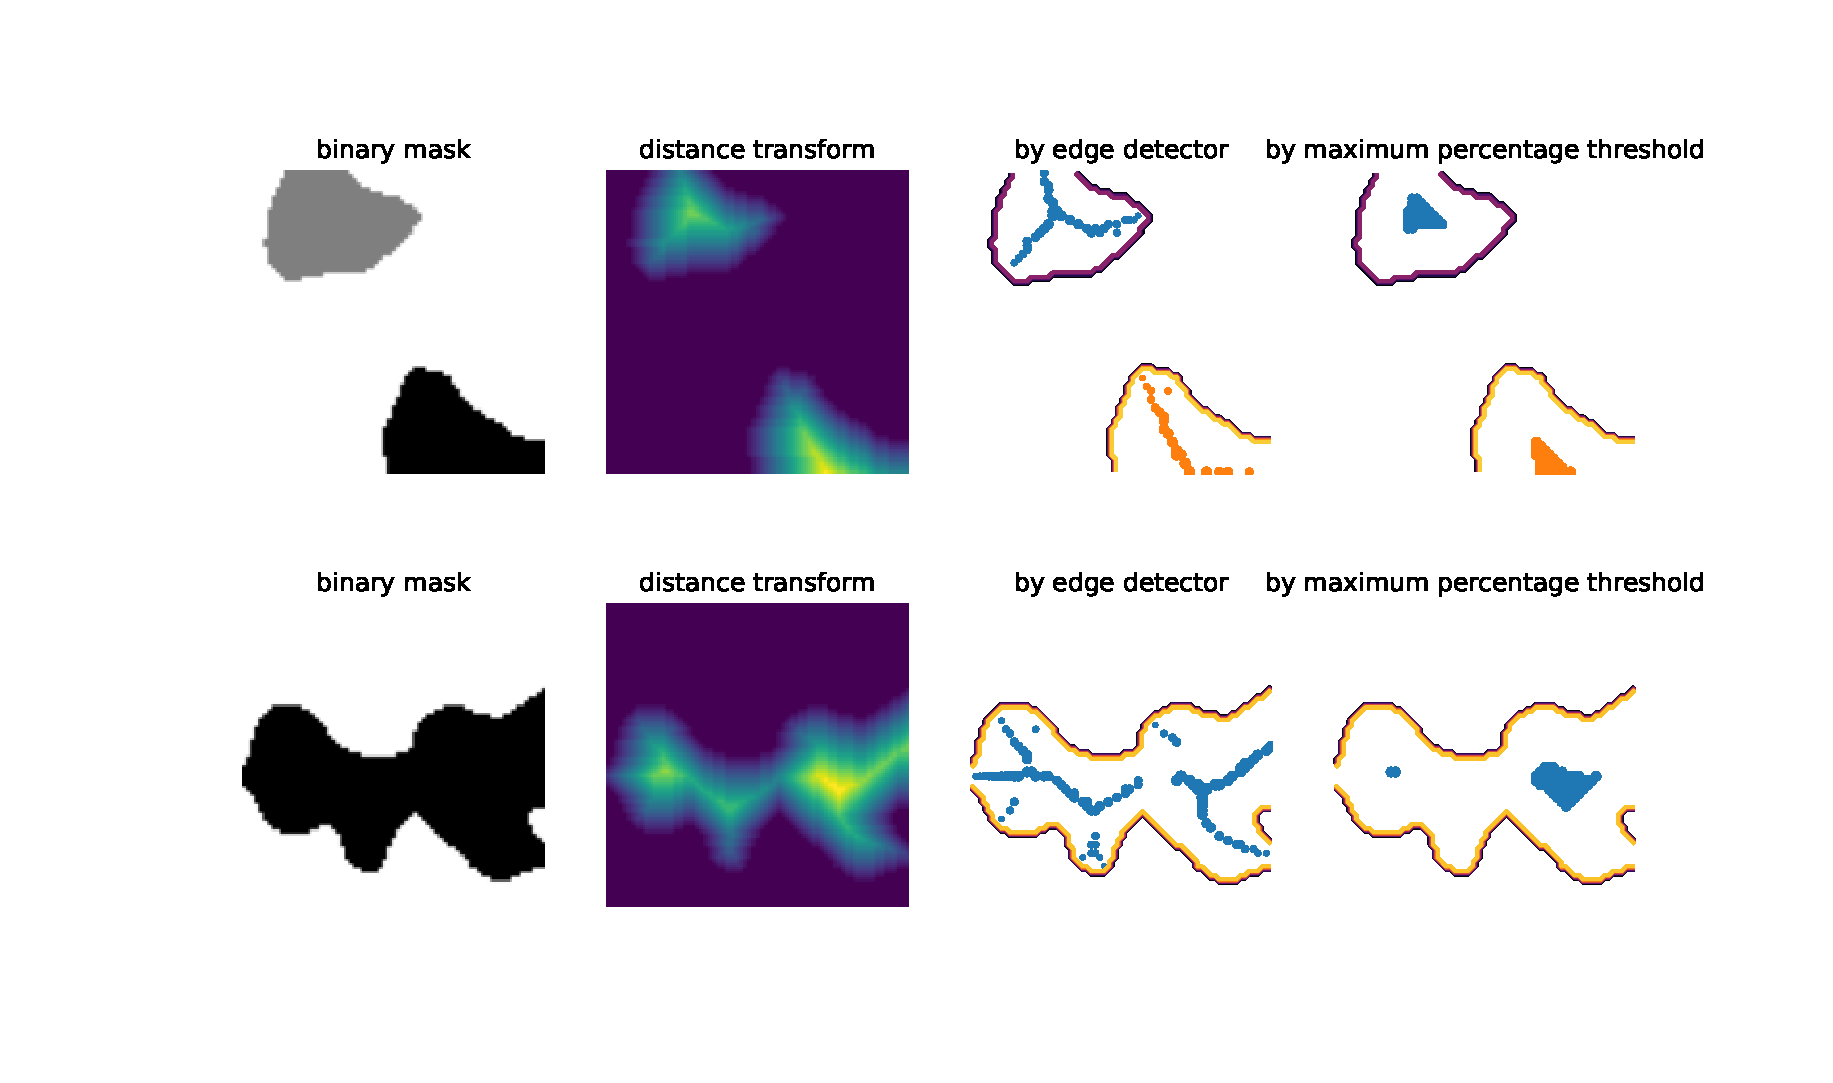
\includegraphics[width=\textwidth]{figures/centralsbyfilter.eps}
  \caption{The first two columns show the original mask and its distance transform result. In the second column, a brighter pixel indicates a higher distance to the background. The third column shows the central points extracted by a edge detector. The fourth column shows central points found by a percentage filter ($> 80\%$) of the highest distance value.}
  \label{fig:DTafterfilter}
\end{figure}

\subsection{Informativity and Stability of Central Points}
Central points preserve most information about the original blob. If the distance value to the background of every central point is preserved, the original blob mask could be approximately recovered from the central points, see \autoref{fig:maskrecover}. In contrary, the shape information is lost when using the centroid representation. Certainly, multiple central points require more memory space than a single centroid, but the central points representation compresses information efficiently. Based on our observation, the ratio of cental points and blob size is around $4\%\sim6\%$: a blob with size 1200 has around 70 central points and a blob with size 500 has around 30 pixels. Therefore, we have reduced the memory usage for every blob by $95\%$ while still kept most information.
\begin{figure}
  \centering
  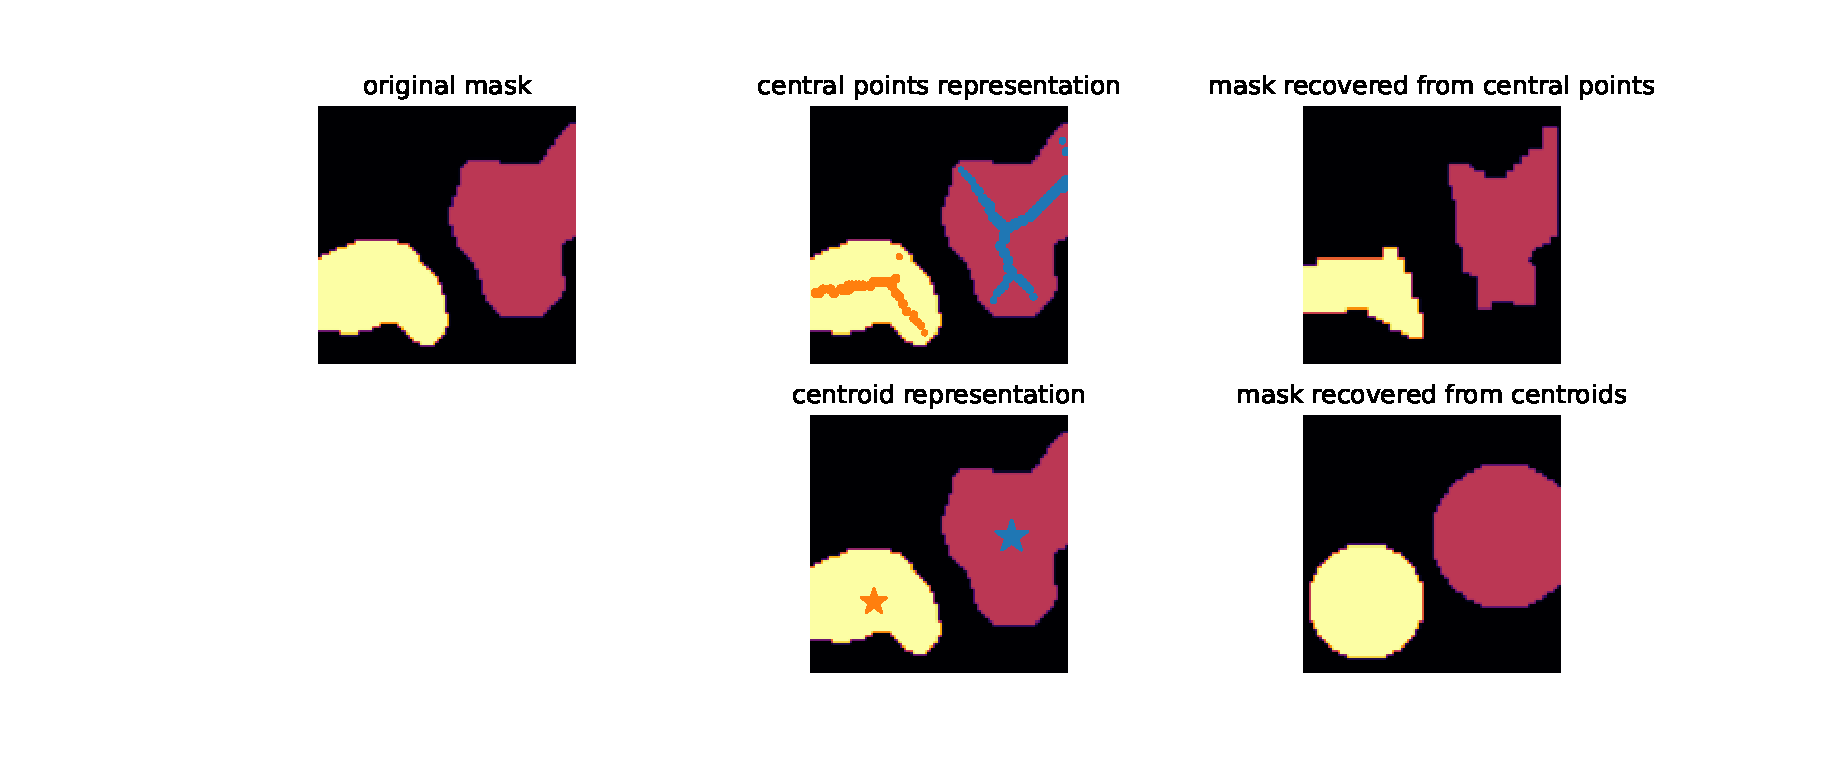
\includegraphics[width=\textwidth]{figures/maskrecover.eps}
  \caption{Mask recovery from the central points shows most of the shape information is preserved}\label{fig:maskrecover}
\end{figure}

The above analysis shows that the central point representation is a stand-alone feature describer, and is independent of the centroid representation. However, because we cannot reduce the number of central points to a low level, the tracking algorithm must find the optimum candidate among all central points, which brings about extra computational cost that is wasted when blobs are not merged. Therefore, we describe the blobs by two representations (see \autoref{eq:blobdenote2}, $P$ is the coordinate of a central point and $D$ is its distance to the background). And would only switch to central points matching if the centroid matching fails. Details about matching are elaborated in \Cref{sec:track}.
\begin{equation}\label{eq:blobdenote2}
  \begin{split}
        B = &\{C,S\}; \\
        &\{(P_1,D_1),(P_2,D_2),\cdots,(P_n,D_n)\}
      \end{split}
\end{equation}

The cluster of central points looks like the ``spine'' of the original blob. This is not surprising because we visually examine the shape of the local maxima points in \autoref{fig:DTafterfilter}. Actually, the set of local maxima points in a distance transform are an approximation to the medial axis of a binary mask \cite{lee1996chessboard}, see \autoref{fig:medialaxisandcentral}. A medial axis of a $R^2$ shape is the set of points that have more than one closest point on the object's contour line. \citeauthor{attali2009stability} \cite{attali2009stability} proved that for shapes in $R^2$, fluctuation of the shape contour only effect part of the branches of the medial axis. This partially explains why the central points stay stable by blob merging/ splitting.
\begin{figure}
  \centering
  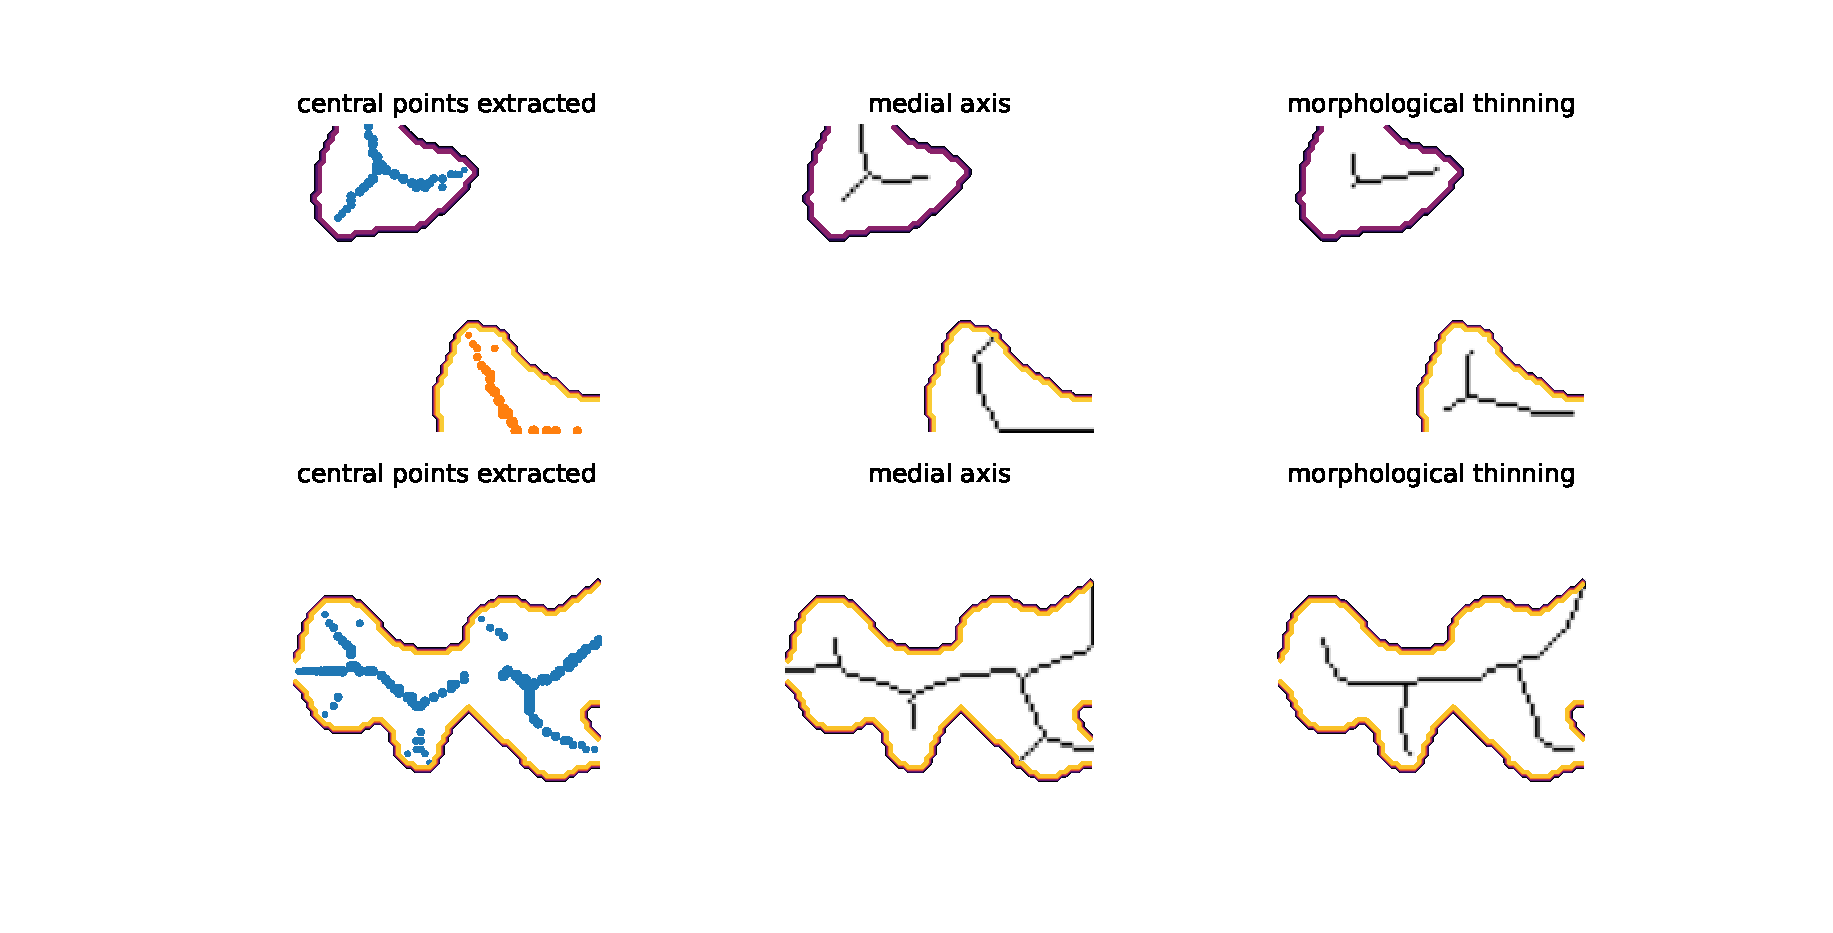
\includegraphics[width=\textwidth]{figures/centralandmedial.eps}
  \caption{The first column shows the set of central points, the second column is the medial axis of the same binary mask. The third column shows result of another thinning algorithm by \cite{zhang1984fast}.}\label{fig:medialaxisandcentral}
\end{figure}



